\section{Experiments}
\subsection{Datasets}
\textbf{Synapse dataset:}  The dataset includes 3779 axial abdominal clinical CT images from 30 cases. Each abdominal CT scan ranges from 85 to 198 CT slices of $512 \times 512$ pixels with voxel spatial resolution of $([0.54\sim 0.54] \times [0.98 \sim 0.98] \times [2.5 \sim 5.0])mm^3$. In this paper, following~\cite{chen2021transunet}, 18 CT case samples are divided into the training set, and the remaining 12 CT case samples are allocated to the test set. The average DSC and HD95 are used as the evaluation metrics to assess the segmentation performance of CA-UNet on 8 abdominal organs: Aorta, Gallbladder, Left Kidney, Right Kidney, Liver, Pancreas, Spleen, and Stomach.

%$\tnofoote{1 https://www.synapse.org/#!Synapse:syn3193805/wiki/217789}$
%$\footnote{2 https://www.creatis.insa-lyon.fr/Challenge/acdc/}$


\textbf{ACDC dataset:}  The dataset collects cardiac magnetic resonance imaging data from different patients using MRI scanners. The slice thickness of each MRI scan case is $5\sim8$ millimeters, covering the entire heart from the base to the top of the left ventricle. Additionally, the planar spatial resolution of these short-axis slices is between $0.83 \times 1.75 mm^2$/pixels. Each MRI scan case slice is professionally annotated in detail, including Left Ventricle (LV), Right Ventricle (LV), and myocardium (Myo). Following~\cite{chen2021transunet}, this dataset is randomly divided into 70 training samples (including 1930 axial slices), 10 validation samples, and 20 test samples. This paper uses average DSC to evaluate the performance of the algorithm proposed in this paper on the segmentation of 3 cardiac tissues.


\subsection{Implementation details}
The CA-UNet is implemented based on PyTorch and is trained and tested on the Nvidia GeForce RTX 4090 GPU. For each batch, the number of samples is set to 16 with a total of 400 iterations. Moreover, in this chapter, the number of channels $C$ of feature maps at all levels of the network model is set to 96, and the network model weights are randomly initialized and retrained. The AdamW optimizer is used, with the learning rate set to 0.001, momentum set to 0.9, and weight decay set to 1e-4. The data augmentation strategy follows MISSFormer~\cite{huang2022missformer}.


\begin{figure}[t!]
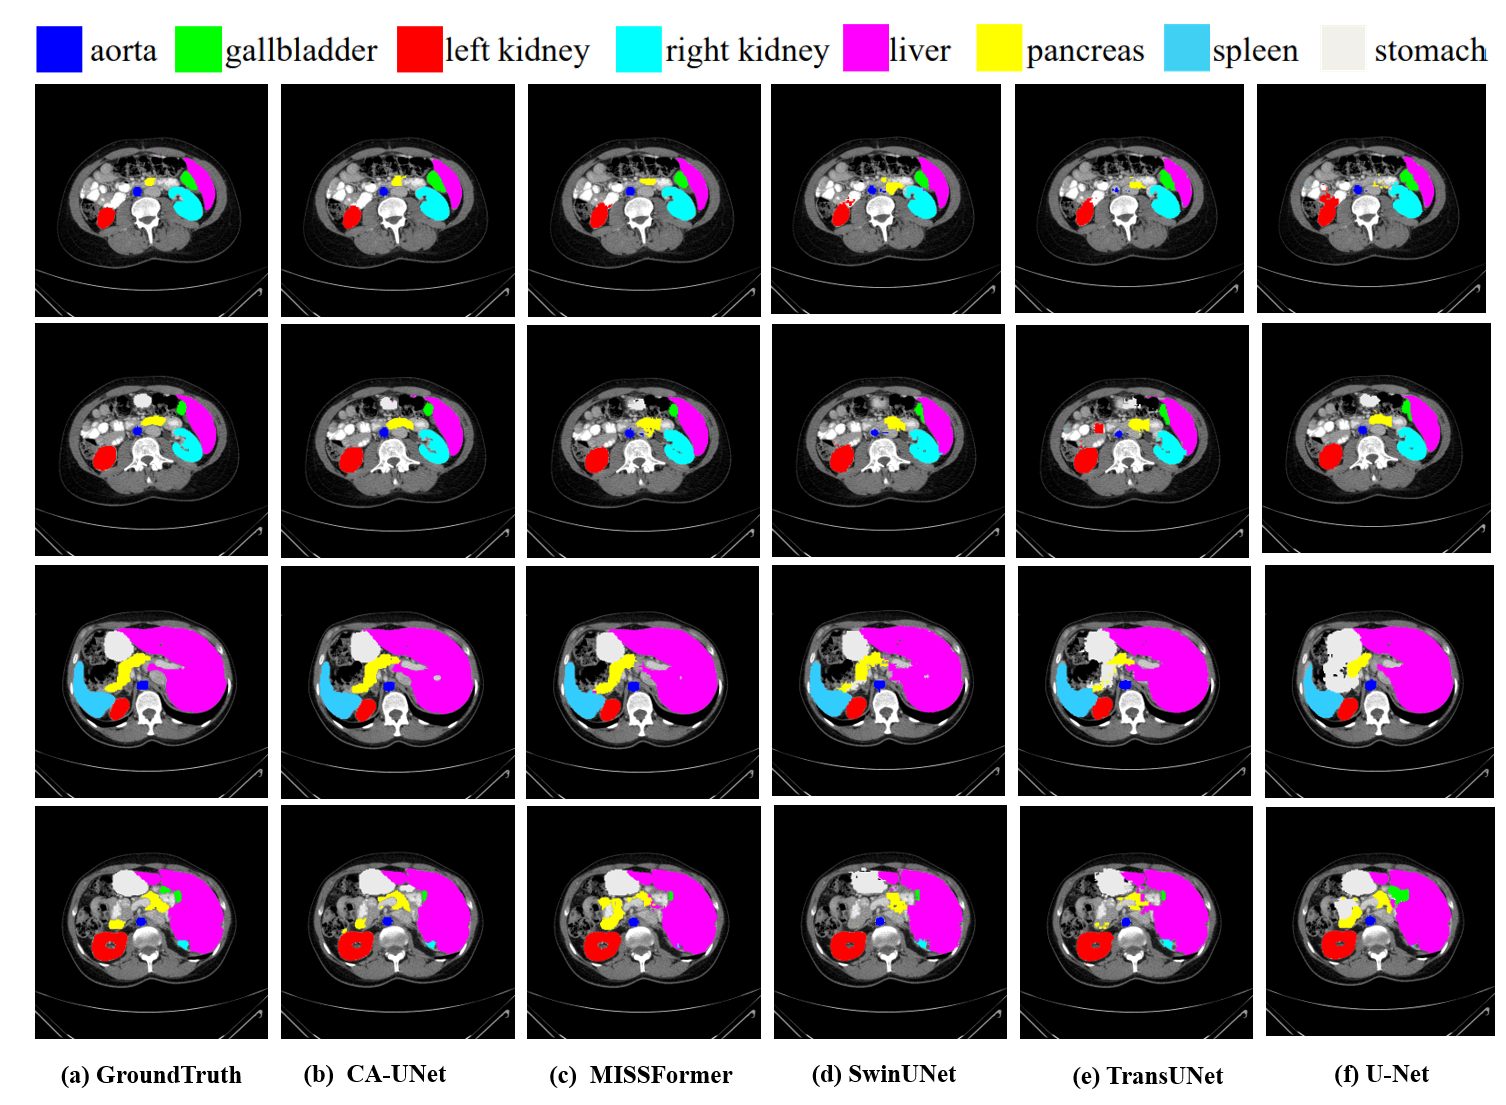
\includegraphics[width=\textwidth]{images/visulisation.png}
\caption{The segmentation visual results of different methods on the Synapse multi-organ CT dataset.}\label{segmentation}
\end{figure}



\subsection{Experiment results on Synapse dataset}

Table.~\ref{synapse} shows the quantitative comparison results of the segmentation accuracy (average DSC and HD95) of CA-UNet with the current mainstream methods.Experimental results demonstrate that our method achieves the best performance with segmentation accuracy of 84.43\%(DSC$\uparrow$) and 15.69($\downarrow$),respectively, showing an improvement of 1.88\% and 7.04\% compared to CASTformer~\cite{huang2022missformer}. Fig.~\ref{segmentation} shows a visual comparison of different methods on the Synapse multi-organ CT dataset. Compared to the current mainstream CNN-ViT or pure Transformer methods, our method demonstrates the excellence of the parallel heterogeneous feature extraction module. Even when substantially reducing the channel dimension of the feature map, it further optimizes the recognition accuracy of various organs and has higher clarity in edge segmentation.

\begin{table*}[htbp]
    \centering
    \caption{Segmentation accuracy of different methods on the Synapse dataset.}
    \footnotesize
    \resizebox{\textwidth}{!}{
    \begin{tabular}{c|cc|cccccccc}
    \hline
    Methods &  DSC$\uparrow$ &HD95$\downarrow$ & Aorta& Gallbladder& Kidney(L)& Kidney(R)& Liver& Pancreas& Spleen& Stomach\\
    \hline
    V-Net~\cite{milletari2016v} & 68.81 & - & 75.34 & 51.87 & 77.10 & 80.75 &
    87.84 & 40.05 & 80.56 & 56.98 \\
    DARR~\cite{fu2020domain} & 69.77 & - & 74.74 & 53.77 & 72.31 & 73.24 &
    94.08 & 54.18 & 89.90 & 45.96 \\
    R50 ViT~\cite{chen2021transunet} & 71.29 & 32.87 & 73.73 & 55.13 & 75.80 &
    72.20 & 91.51 & 45.99 & 81.99 & 73.95 \\
    R50 U-Net~\cite{chen2021transunet} & 74.68 & 36.87 & 84.18 & 62.84 & 79.19 &
    71.29 & 93.35 & 48.23 & 84.41 & 73.92 \\
    U-Net~\cite{ronneberger2015u} & 76.85 & 39.70 & 89.07 & 69.72 & 77.77 & 68.60 &
    93.43 & 53.98 & 86.67 & 75.58 \\
    TransUNet~\cite{chen2021transunet} & 77.48 & 31.69 & 87.23 & 63.13 & 81.87 &
    77.02 & 94.08 & 55.86 & 85.08 & 75.62 \\
    Att-UNet~\cite{oktay2018attention} & 77.77 & 36.02 & \textbf{89.55} & 68.88 & 77.98 &
    71.11 & 93.57 & 58.04 & 87.30 & 75.75 \\
    Swin UNet~\cite{cao2022swin} & 79.13 & 21.55 & 85.47 & 66.53 & 83.28 &
    79.61 & 94.29 & 56.58 & 90.66 & 76.60 \\
    MISSFormer~\cite{huang2022missformer} & 81.96 & 18.20 & 86.99 & 68.65 & 85.21 &
    82.00 & 94.41 & 65.67 & 91.92 & 80.81 \\
    CASTformer~\cite{you2022class} & 82.55 & 22.73 & 89.05 & 67.48 & 86.05 &
    82.17 & \textbf{95.61} & 67.49 & 91.00 & 81.55 \\
    \hline
    CA-UNet & \textbf{84.43} & \textbf{15.69} & 88.59 & \textbf{73.70} & \textbf{87.92} & \textbf{83.34} & 94.85 & 
    \textbf{71.52} & \textbf{91.98} & \textbf{82.51} \\
    \hline
    \end{tabular}
    }
    \label{synapse}
    \end{table*}


\subsection{Experiment results on ACDC dataset}

To validate the robustness and generalizability of CT-UNet on other medical datasets, we conducted training on the ACDC dataset in MRI mode, with experimental results shown in Table.~\ref{acdc}. The CA-UNet we proposed achieved 90.68\% accuracy in the segmentation of three types of cardiac tissues. The experimental results show that our method has reached an advanced level in the segmentation of Myo, while the segmentation performance for the LV and RV also reached a level comparable to the current mainstream method.
  
\begin{table}[htbp]
\caption{Segmentation accuracy of different methods on the ACDC dataset.}\label{acdc}
\begin{tabular}{c|c|ccc}
\hline
Methods & DSC& RV & Myo& LV\\
\hline
R50-U-Net~\cite{chen2021transunet} & 87.55 & 87.10 & 80.63 & 94.92\\
R50-AttnUNet~\cite{chen2021transunet} & 86.75 & 87.58 & 79.20 & 93.47\\
ViT-CUP~\cite{chen2021transunet} & 81.45 & 81.46 & 70.71 & 92.18\\
R50-ViT-CUP~\cite{chen2021transunet} & 87.57 & 86.07 & 81.88 & 94.75\\
TransUNet~\cite{chen2021transunet} & 89.71 & \textbf{88.86} & 84.53 & 95.73\\
Swin UNet~\cite{cao2022swin} & 90.00 & 88.55 & 85.62 & \textbf{95.83} \\
\hline
CA-UNet & \textbf{90.68} & 88.57 & \textbf{89.83} & 93.63 \\
\hline
\end{tabular}
\centering
\end{table}


\subsection{Ablation study}

Our proposed CA-UNet effectively aggregates a parallel heterogeneous module that fuses convolution and attention mechanisms, residual-structure-based downsampling, and full-scale skip connection based on CBAM. As a result, it demonstrates superior segmentation performance and generalization ability in medical imaging segmentation tasks. To verify its rationality and effectiveness, we conducted the following ablation experiment on the Synapse dataset.

\subsubsection{Effect of the parallel heterogeneous module:}

CA-UNet combines DwConv and self-attention in SwinTransformer to construct a parallel heterogeneous module for network hierarchical feature extraction and fusion, dynamically allocating weights adaptively in spatial position and channel dimensions. To verify its effectiveness, we examined whether the introduction of negligible computational cost deep convolution (for channel dimension feature capture) has an impact on segmentation performance. The ablation experiment results in Table.~\ref{phb} show that the average DSC of various organ segmentations was increased from 77.82\% to 84.43\%, a 3.97\% increase, through the designed hierarchical parallel heterogeneous module. This effectively enhances the recognition capability of complex medical image organs, making the edge segmentation more precise.

\begin{table}[htbp]
\caption{Ablation study on the effect of the parallel heterogeneous module:}\label{phb}
\footnotesize
\resizebox{\textwidth}{!}{
\begin{tabular}{c|c|cccccccc}
\hline
Methods &  DSC & Aorta& Gallbladder& Kidney(L)& Kidney(R)& Liver& Pancreas& Spleen& Stomach\\
\hline
$-$ DwConv & 80.38 & 87.54 & 68.35 & 78.77 & 77.48 & 93.99 & 66.53 & 89.43 & 80.93\\
$+$ DwConv & \textbf{84.43} & \textbf{88.59} & \textbf{73.70} & \textbf{87.92} & \textbf{83.34} & \textbf{94.85} & \textbf{71.52} & \textbf{91.98} & \textbf{82.51} \\
\hline
\end{tabular}
}
\centering
\end{table}

\subsubsection{Effect of downsampling module based on Res block:}

We incorporated the residual structure into the downsampling module, effectively enhancing the key detail features of the encoder feature maps at all scales and effectively avoiding the issue of feature location information loss caused by traditional downsampling methods (average pooling and max pooling). To validate its effectiveness, we explored the impact of using max pooling and Res block for downsampling on the segmentation performance of CA-UNet. The ablation experiment results in Table.~\ref{down} show that better segmentation precision was achieved through the downsampling module based on Res block, raising the average DSC from 79.55\% to 84.43\%.

\begin{table}[htbp]
\caption{Ablation study on the effect of downsampling module based on Res block}\label{down}
\footnotesize
\resizebox{\textwidth}{!}{
\begin{tabular}{c|c|cccccccc}
\hline
Downsampling &  DSC & Aorta& Gallbladder& Kidney(L)& Kidney(R)& Liver& Pancreas& Spleen& Stomach\\
\hline
Max pooling & 82.56 & 88.54 & 69.94 & 87.18 & 81.57 & 94.72 & 67.34 & 90.19 & 80.98\\
Residual structure & \textbf{84.43} & \textbf{88.59} & \textbf{73.70} & \textbf{87.92} & \textbf{83.34} & \textbf{94.85} & \textbf{71.52} & \textbf{91.98} & \textbf{82.51} \\
\hline
\end{tabular}
}
\centering
\end{table}

\subsubsection{Effect of the full-scale skip connection base on CBAM:}

We introduced a full-scale skip connection based on CBAM, which autonomously learns and aggregates the feature information of all levels of the encoder through spatial and channel attention, reducing the semantic gap caused by the blurring of feature mapping between the encoder and decoder. To explore its effectiveness, we discussed the impact of traditional skip connection based on channel dimension concatenation(CDC) and full-scale skip connection based on CBAM on network segmentation performance. The experimental results in Table.~\ref{skip} show that by introducing a full-scale skip connection based on CBAM, the segmentation accuracy of CA-UNet is effectively improved, raising the average DSC from 78.29\% to 84.43\%.

\begin{table}[htbp]
    \caption{Ablation study on the effect of downsampling module based on the residual structure}\label{skip}
    \footnotesize
    \resizebox{\textwidth}{!}{
    \begin{tabular}{c|c|cccccccc}
    \hline
    skip connection &  DSC & Aorta& Gallbladder& Kidney(L)& Kidney(R)& Liver& Pancreas& Spleen& Stomach\\
    \hline
    CDC & 80.09 & 87.11 & 70.45 & 79.35 & 74.11 & 94.34 & 63.53 & 90.16 & 81.69\\
    CBAM & \textbf{84.43} & \textbf{88.59} & \textbf{73.70} & \textbf{87.92} & \textbf{83.34} & \textbf{94.85} & \textbf{71.52} & \textbf{91.98} & \textbf{82.51} \\
    \hline
    \end{tabular}
    }
    \centering
    \end{table}

% \begin{table}[t!]
% \caption{Ablation study on the impact of the input size}\label{input}
% \footnotesize
% \resizebox{\textwidth}{!}{
% \begin{tabular}{c|c|cccccccc}
% \hline
% Input size &  DSC& Aorta& Gallbladder& Kidney(L)& Kidney(R)& Liver& Pancreas& Spleen& Stomach\\
% \hline
% 224 &  79.13& 85.47&66.53&83.28&79.61&94.29&56.58&\textbf{90.66}&\textbf{76.60}\\
% 384 &  \textbf{81.12} & \textbf{87.07}&\textbf{70.53}&\textbf{84.64}&\textbf{82.87}&\textbf{94.72}&\textbf{63.73}&90.14&75.29\\
% \hline
% \end{tabular}
% }
% \centering
% \end{table}

% \subsubsection{Effect of input size:}
% The testing results of the proposed Swin-Unet with $224\times224$, $384\times384$ input resolutions as input are presented in Table.~\ref{input}. As the input size increases from $224\times224$ to $384\times384$ and the patch size remains the same as $4$, the input token sequence of Transformer will become larger, thus leading to improve the segmentation performance of the model. However, although the segmentation accuracy of the model has been slightly improved, the computational load of the whole network has also increased significantly. In order to ensure the running efficiency of the algorithm, the experiments in this paper are based on $224\times224$ resolution scale as the input.


% \subsection{Discussion}

% As we all known, the performance of Transformer-based model is severely affected by model pre-training. In this work, we directly use the training weight of Swin transformer~\cite{swin} on ImageNet to initialize the network encoder and decoder, which may be a suboptimal scheme. This initialization approach is a simple one, and in the future we will explore the ways to pre-train Transformer end-to-end for medical image segmentation. Moreover, since the input images in this paper are 2D, while most of the medical image data are 3D, we will explore the application of Swin-Unet in 3D medical image segmentation in the following research.







